%!TEX root = ../crowd_hierarchies_kdd.tex

% THIS IS AN EXAMPLE DOCUMENT FOR VLDB 2012
% based on ACM SIGPROC-SP.TEX VERSION 2.7
% Modified by  Gerald Weber <gerald@cs.auckland.ac.nz>
% Removed the requirement to include *bbl file in here. (AhmetSacan, Sep2012)
% Fixed the equation on page 3 to prevent line overflow. (AhmetSacan, Sep2012)


\section{Introduction}
\label{sec:intro}

The recent vogue of extracting and categorizing disorganized information from various sources into centralized knowledge bases, taxonomies and structured data repositories has revolutionized many applications, including search and question answering~\cite{kngraph}, event monitoring and prediction~\cite{leetaru2013gdelt,Leban:2014} and recommendation systems~\cite{burke,Adomavicius:2005}. Nevertheless, most existing efforts to extract and collect information in repositories of organized data focus on {\em head data} - data about popular entities, facts, etc. -  leaving behind a considerable volume of fine-grained data belonging in the {\em long tail}, i.e., data about less popular entities, less popular facts and so on. Thus, it is of the utmost importance to tap into the long tail to get the most of available knowledge assets and collective expertise.

One of the most promising directions towards the conquest of long tail data is that of combining human computation with traditional computation, commonly referred to as {\em crowdsourcing}. Crowdsourcing is not a cheap way to outsource work to volunteers. However, when done right, it is an entire new form of {\em fine-grained knowledge production} with the potential to revolutionize many application domains ranging from imagine processing to traditional database and data curation systems. and data integration systems ~\cite{quinn-crowdsourcing, vox-populii, doan2011crowdsourcing, ribeiro11, deco, qurkCIDR, crowddb, tamer, franklin:2011, Parameswaran:2012, west:2014}.

Consequently, the problem of {\em crowdsourced entity extraction}, i.e., extracting and collecting entities from the crowd and building organized data catalogs, has gained increasing attention recently~\cite{trushkowsky:2013, amsterdamer:2014, park:2014, kondredi:2014}. Most existing approaches for crowdsourced entity extraction focus on {\em microtasked}-based approaches and rely on repeatedly asking the same query to workers. For example, given the task of collecting all events, such as concerts, rallies, etc., in Greece, current techniques focus on asking workers to ``list one more event in Greece'' repeatedly until a sufficient level of {\em completeness}, i.e., number of distinct entities, is achieved. The latter is rather challenging as we assume an ``open world''~\cite{franklin:2011} and absence of ground-truth information.

Existing approaches~\cite{trushkowsky:2013} focus on devising techniques for estimating the completeness of the extraction result but startlingly fail to directly optimize (i.e., minimize) the total cost of extraction. In fact, issuing the same query repeatedly results in large numbers of duplicate extractions in most real-world scenarios. This is due to the fact that popular entities are provided by many workers, leading to increased duplicates, with the less popular entities not being as prevalent in the set of extracted entities. Large numbers of duplicate extractions increase the total cost of corwdsourced entity extraction significantly and can deem crowdsourced extraction impractical for large-scale applications. 

The situation only becomes worse when entities follow a skewed, long tail {\em popularity distribution}, i.e., a small number of entities have significantly higher probability of appearing in worker answers while a large number of {\em rare} entities have minuscule probability of being extracted. Next, we consider two crowdsourced entity extraction applications to demonstrate the presence of long tail popularity distributions and exemplify how they can lead to increased numbers of duplicate extractions.

\begin{figure*}
	\centering
	\subfigure[Event popularity in EventBrite.]{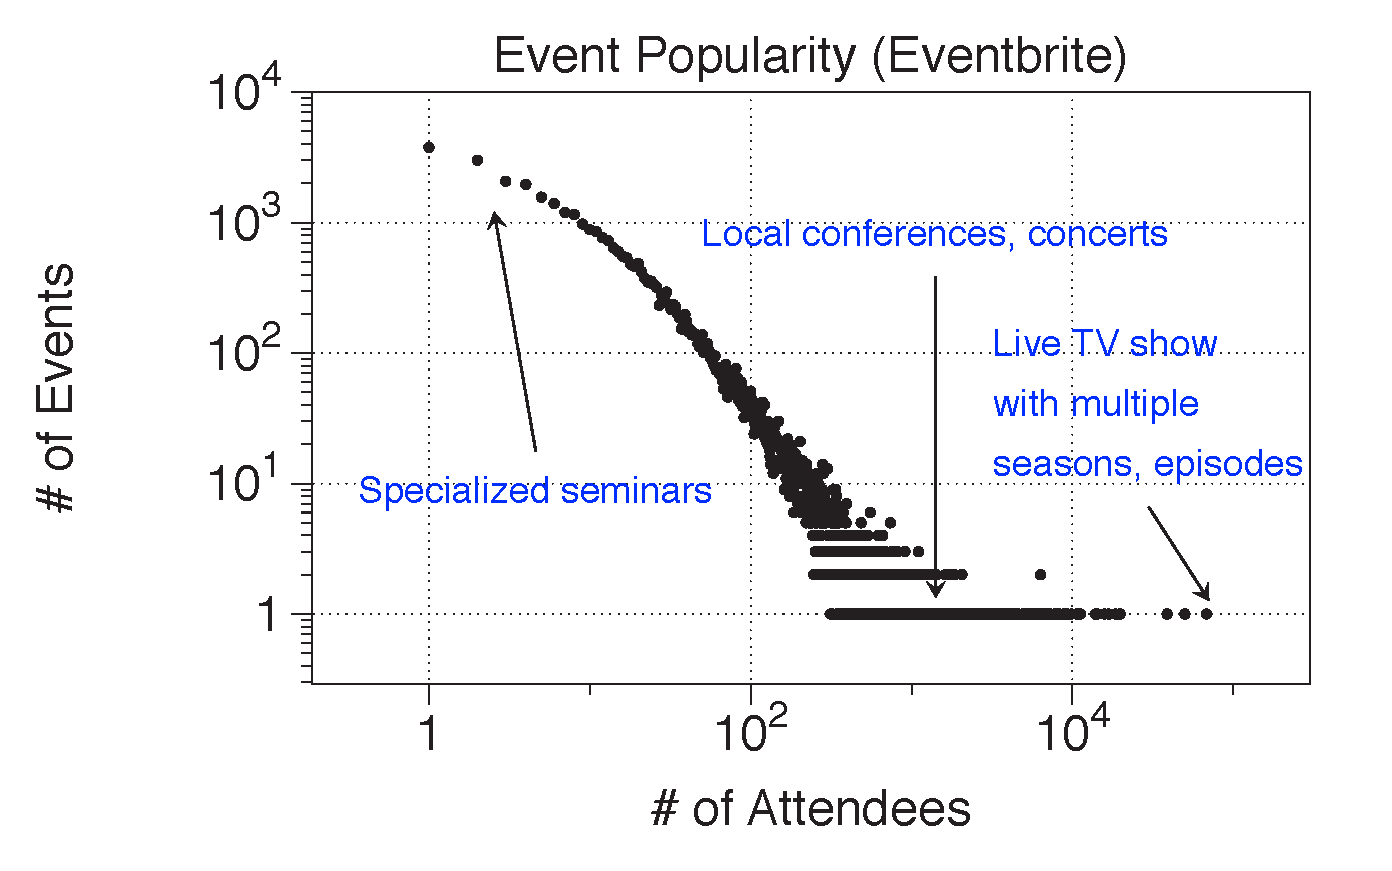
\includegraphics[clip,scale=0.35]{figs/eventPop.eps}\label{fig:eventPop}}
	\subfigure[Entity popularity in crowdsourced people extraction.]{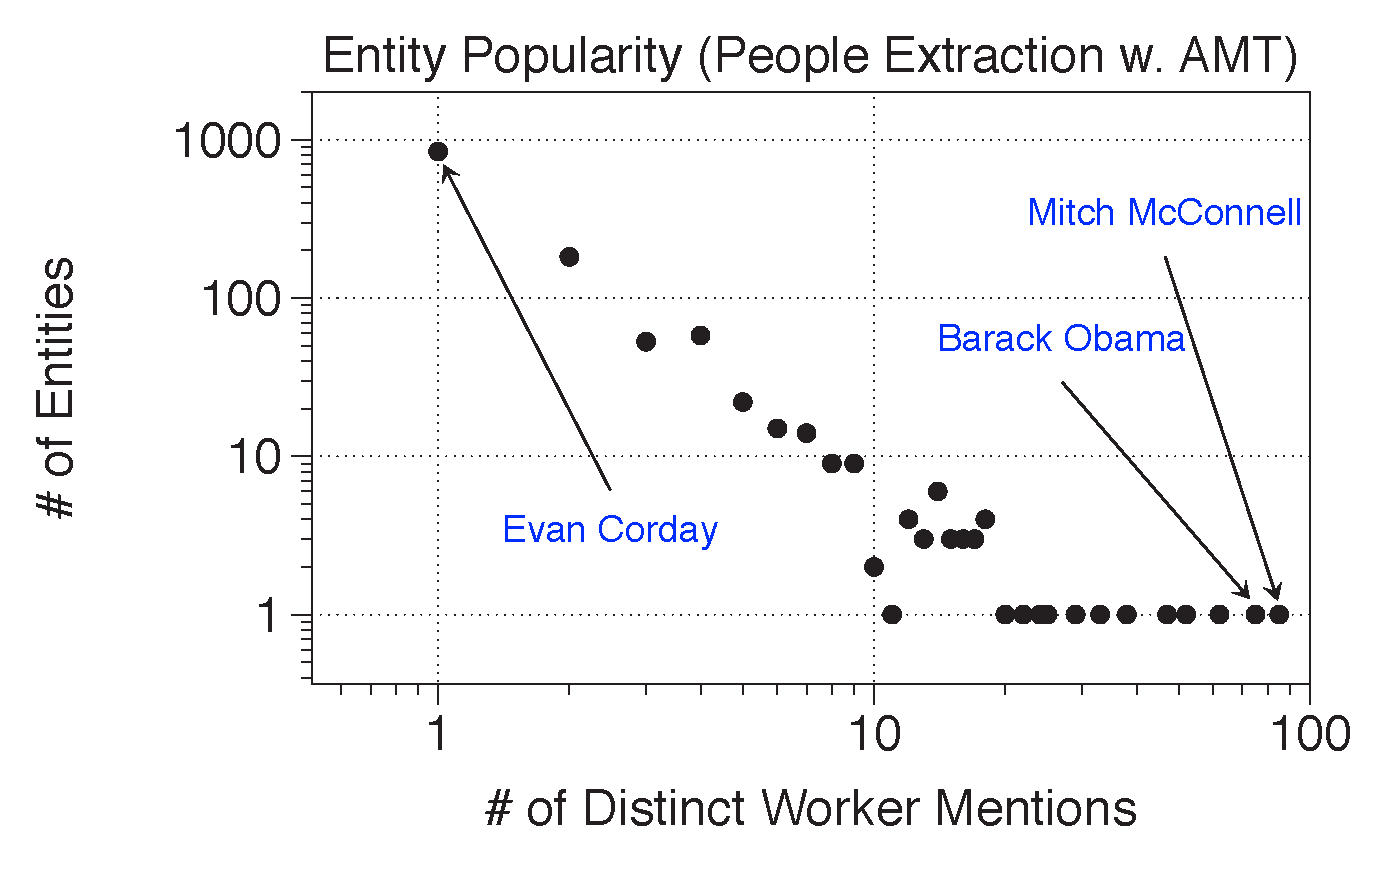
\includegraphics[clip,scale=0.35]{figs/amtPop.eps}\label{fig:amtPop}}
	\caption{Entity popularity distributions exhibit long tails in real crowdsourced entity extraction applications.}
\end{figure*}

\begin{example}
First, we consider Eventbrite~(\url{www.eventbrite.com}), an online event aggregator, that relies on crowdsourcing to compile a directory of events with detailed information about the location, type, date and category of each event. We collected a dataset via Eventbrite's API with events of 19 different categories from 63 different countries over a time period of 31 days. To measure the popularity of each event we use as a surrogate the number of attendees that registered for a specific event via Eventbrite.  In \Cref{fig:eventPop} we plot the number of registered attendees for different events grouping together events that had the same number of attendees. As shown, there is a large number of events with less than 100 attendees corresponding mostly to specialized seminars, and a small number of extremely popular events corresponding to concerts or live TV shows. 
\end{example}

As we did not have immediate access to crowd workers for the aforementioned application, we also conducted a real crowdsourcing experiment via Amazon's Mechanical Turk (AMT)~\cite{mturk} that allowed us to precisely measure the popularity of extracted entities. 

\begin{example}
We asked workers to list ``people in the news''. In particular, we asked them to consider five major online US news portals, ``New York Times'', ``Huffington Post'', ``Washington Post'', ``USA  Today'' and ``The Wall Street Journal'', and report five distinct people per HIT. We issued 600 HITs for \$0.20 per HIT served by 143 unique workers. To ensure the accuracy of our results we asked workers to provide us with a link corresponding to the extraction. These links were manually verified.  In total, we extracted 1,245 unique people. \Cref{fig:amtPop} shows the number of distinct workers that reported each person. As shown, there are 12 people that were reported by at least 20 different workers but there is a long tail of 842 people that were reported by one worker and 182 people reported by two workers. 
\end{example}

\noindent\textbf{Our approach.} In this paper, our goal is to {\em make crowdsourced entity extraction practical}. Unlike previous work, we focus on the problem of {\em budgeted crowdsourced entity extraction}, where we are given a budget and we want to maximize the number of retrieved entities; we believe this is a more practical goal, instead of the goal of retrieving all entities.  Effectively our goal is to minimize the total cost spent on duplicate extractions and maximize the total number of extracted entities. To do so, we focus on entity extraction over {\em structured domains}, i.e., domains that can be fully described by a collection of attributes, each potentially exhibiting hierarchical structure, and demonstrate how exploiting the domain's structure can help us achieve the aforementioned goal. We point out that often the structure of domains in practical applications is already known by design. For example, Eventbrite categorizes extracted events based on a location taxonomy, an event type and their date. 

Leveraging this structure we use a much richer space of crowd queries, thus, we avoid issuing the same query repeatedly. More precisely, if we view the structured data domain as a \emph{partially ordered set} (poset), then each query can be mapped to a node in the graph describing its topology. This allows for more targeted queries, e.g., ``list an electro-swing concert in Greece'', and enables us to explore a larger space of entities effectively by focusing on diverse and potentially disjoint groups of entities. Moreover, we extend typical crowd queries to also include an {\em exclude list}, e.g., ``list an electro-swing concert in Greece that is not by Parov Stelar''. Both aforementioned approaches allow us to effectively reduce the number of duplicate extractions and enable us to extract more entities from the underlying domain (see \Cref{sec:exps}).

The ability to ask richer queries comes with a host of new challenges. First and foremost, we need to address the fundamental question: {\em Which is the most profitable query to issue next?}. For this, we propose a collection of  statistical techniques for estimating the {\em gain} of further queries, i.e., the number of new distinct entities extracted, for any node in the poset. Our techniques make use of the extracted entities by previously issued queries to derive accurate estimates for new queries corresponding to the nodes of the poset.  

However, the input poset is of exponential size with respect to the number of attributes describing the domain. This, leads to additional challenges in deciding which queries to issue: (a)~{\em Sparsity:} Many of the nodes in the poset are likely to be empty, i.e., the queries corresponding to those nodes are likely to not have any answers; avoiding asking queries corresponding to these nodes is essential to keep monetary cost low. (b)~{\em Limited information:} The larger the poset the fewer the observed entities corresponding to lower level nodes in the poset, thus, we only have limited information when estimating the gain of further queries at these nodes.  (c)~{\em Interrelationships:} Many of the nodes in the poset are ``coupled'' with one another; for example, the results from a few queries corresponding to ``list a concert in Greece'' can inform whether issuing queries corresponding to ``list a rock concert in Greece'' is useful or not. 

In summary, our main contributions are as follows:
\squishlist
\item We formalize the notion of {\em generalized queries} that ask workers to provide us with entities from a domain $D$ and can also include an {\em exclude list}. In general such queries are of the type ``Give me $k$ more entities with attributes $\bar{X}$ that belong in domain $D$ and are not in $\{A, B, ...\}$''.  Extending techniques from the species estimation and building upon the multi-armed bandits literature, we introduce a new methodology for estimating the gain for generalized queries. 
\item We propose a novel algorithmic framework that exploits the structure of the entity extraction domain to maximize the number of extracted entities under given budget constraints by targeting tail entities. In particular, we view the problem of entity extraction as a {\em multi-round adaptive optimization problem}. At  each round we exploit the information on extracted entities obtained by previous queries to adaptively select the crowd query that will maximize the {\em cost-gain} trade-off at each round. 
\item We develop a new technique to estimate the gain of generalized entity extraction queries under the presence of little information, i.e., only when a small portion of the underlying entity population has been observed. We empirically demonstrate its effectiveness when extracting entities from sparse domains.
\item Finally, we show that our techniques can effectively solve the problem of budgeted crowd entity extraction for large data domains on both real-world and synthetic data.
\squishend

%Our main contributions are as follows:
%
%\squishlist
%\item We formalize the notion of an exclude list for crowdsourced entity extraction queries and show how previously proposed gain estimators can be extended to handle such queries.
%\item We develop a new technique to estimate the gain of generalized entity extraction queries under the presence of little information, i.e., only when a small portion of the underlying entity population has been observed. We empirically demonstrate its effectiveness when extracting entities from sparse domains.
%\item We introduce an adaptive optimization algorithm that takes as input the gain estimates for different types of queries and identifies querying policies that maximize the total number of retrieved entities under given budget constraints. 
%\item Finally, we show that our techniques can effectively solve the problem of budgeted crowd entity extraction for large data domains on both real-world and synthetic data.
%\squishend

%Previously proposed techniques~\cite{trushkowsky:2013} do not directly apply to the scenario where we are traversing a poset corresponding to this structured data domain, and new techniques are needed. The main limitation of the aforementioned techniques is that they focus on estimating the completeness of a specific fixed query and are agnostic to cost. As a consequence they do not address the problem of deciding which additional queries are \emph{worth} issuing.  To mitigate these shortcomings, one needs to tune the queries that are asked. However, deciding which queries to ask among a large number of possible queries (exponential in the number of attributes describing the input domain) and when and how many times to ask each query, are both critical challenges that need to be addressed. Furthermore, unlike previous work, we focus on the budgeted case, where we are given a budget and we want to maximize the number of retrieved entities; we believe this is a more practical goal, instead of the goal of retrieving all entities.  


%
%
%\iftr
%Our crowdsourced entity extraction techniques can be useful for a variety of entity extraction applications that are naturally coupled to a structured domain, including:
%\squishlist
%\item A newspaper that wants to collect a list of today's events to be displayed on the events page every day. 
%In this case, the structured data domain could include event type (e.g., music concerts vs.~political rallies) or location, among other attributes.
%\item A stock trading firm wants to collect a list of stocks that have been mentioned by popular press on the previous day. In this case, the structured data domain could include stock type, popular press article type, or whether the mention was positive or negative, among other attributes. 
%\item A real estate expert wants to curate a list of houses available for viewing today. The structured data domain in this case could include the price range, the number of floors, etc.
%\item A university wants to find all the faculty candidates on the job market. The structured data domain in this scenario includes the university of the applicant, specialization, and whether they are Ph.D./Postdoc.
%\item The PC chair of a new conference wants to find potential reviewers. The domain describing each of the candidates can be characterized by the university or company of the reviewer, expertise, qualifications, and so on. 
%\squishend
%\fi
%
%\subsection{Challenges in Structured Domains}
%\label{sec:challenges}
%To exemplify the aforementioned challenges we review a large-scale real-world scenario where crowdsourcing is used to extract entities. We consider Eventbrite~(\url{www.eventbrite.com}), an online event aggregator, that relies on crowdsourcing to compile a directory of events with detailed information about the location, type, date and category of each event. \iftr Typically, event aggregators are interested in collecting information about diverse events spanning from conferences and music festivals to political rallies across different location, i.e., countries or cities. In particular, \fi Eventbrite collects information about events across different countries in the world. Each country is split into cities and areas across the country. Moreover, events are organized according to their type and topic. The attributes and their corresponding structure are known in advance and are given by the design of the application. \iftr We collected a dataset from Eventbrite spanning over 63 countries that are divided into 1,709 subareas (e.g., states) and 10,739 cities, containing events of 19 different types, such as rallies, tournaments, conferences, conventions, etc. and a time period of 31 days spanning over the months of October and November. \fi
%
%Two of the three dimensions, i.e., location and time, describing the domain of collected events  are hierarchically structured. The poset characterizing the domain can be fully specified if we consider the cross product across the possible values for location, event type and time. For each of the location, time, type dimensions we also consider a special {\em wildcard} value. Taking the cross-product across the possible values of these dimensions results in poset with a total of 8,508,160 nodes containing 57,805 distinct events overall. We point out that the events associated with a node in the poset overlap with the events corresponding to its descendants. First, we demonstrate how the sparsity challenge applies to Eventbrite.
%\begin{example}
%We plot the number of events for each node in the poset describing the Eventbrite domain. Out of 8,508,160 nodes only 175,068 nodes are associated with events while the remaining have zero events. \Cref{fig:eventbritepop} shows the number of events per node (y-axis is in log-scale). Most of the populated nodes have less than 100 events. Additionally, the most populated nodes of the domain correspond to nodes at the higher levels of the poset. When extracting events from such a sparse domain one needs to carefully decide on the crowdsourced queries to be issued especially if operating under a monetary budget.
%\end{example}
%\iftr
%\begin{figure}
%	\begin{center}
%	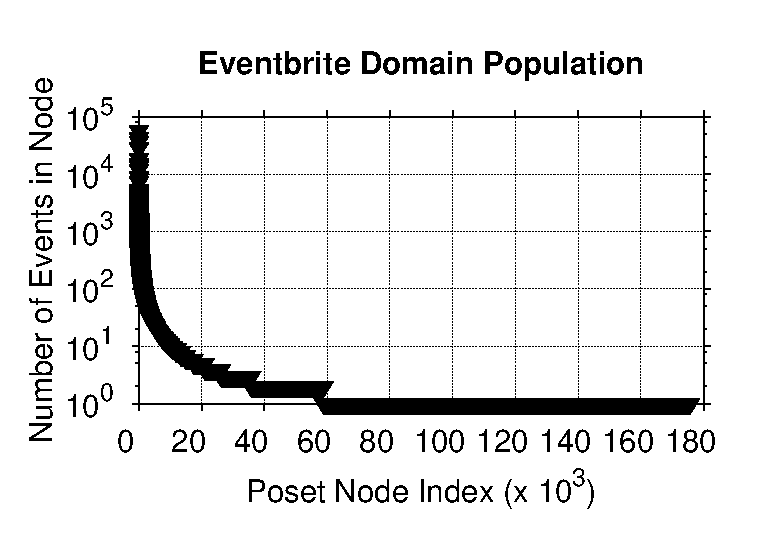
\includegraphics[clip,scale=0.5]{figs/eventbritepop.eps}
%	\vspace{-10pt}
%	\caption{The population of different nodes in the Eventbrite domain.}
%	\label{fig:eventbritepop}
%	\vspace{-10pt}
%	\end{center}
%\end{figure}
%\fi
%
%\ifpaper
%\begin{figure}[h]
%	\centering
%	\vspace{-10pt}
%	\subfigure{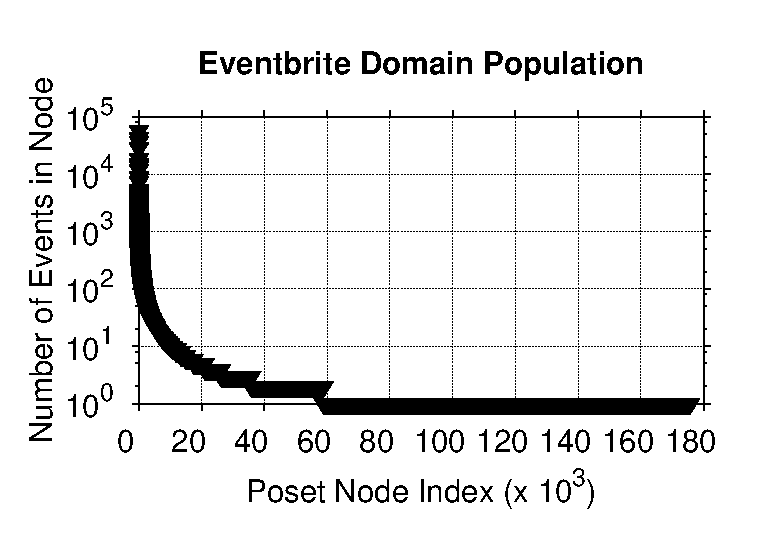
\includegraphics[clip,scale=0.32]{figs/eventbritepop.eps}\label{fig:eventbritepop}}
%	\hspace{-10pt}
%	\subfigure{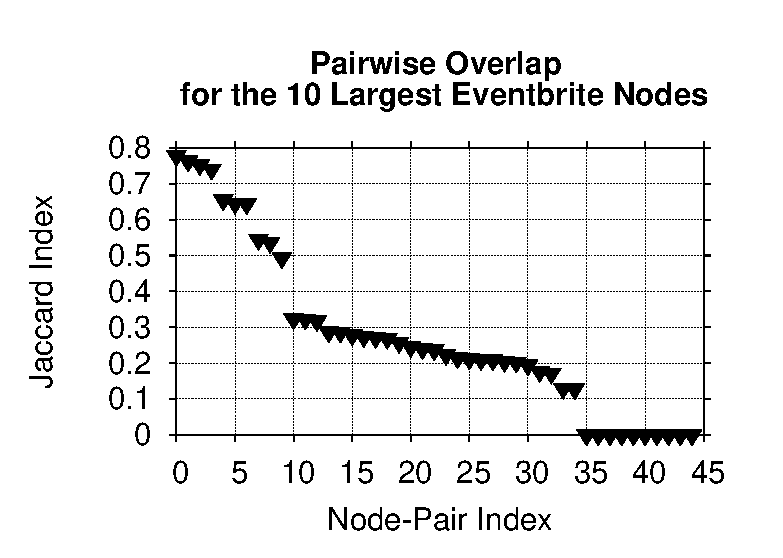
\includegraphics[clip,scale=0.32]{figs/overlaps.eps}\label{fig:eventbriteover}}
%	\vspace{-10pt}
%	\caption{(a) The population of different nodes and (b) pairwise overlaps for the 10 most populous nodes in the Eventbrite domain.}
%	\vspace{-10pt}
%\end{figure}
%\fi
%
%As mentioned before, a critical challenge in such large domains is deciding on the queries to ask. However, the hierarchical structure of the data domain presents us with an opportunity. One approach would be to perform a top-down traversal of the poset and issue queries at the different nodes. Nevertheless, this gives rise to a series of challenges: (i) how can one decide on the number of queries to be asked at each node, (ii) when should one progress to deeper levels of the poset and (iii) which subareas should be explored. We elaborate on these in \Cref{sec:prelims}. Next, we focus on the second challenge, i.e., the interdependencies across poset nodes. 
%\begin{example}
%We consider again the Eventbrite dataset and plot the pairwise overlaps of the ten most populous nodes in the domain. \Cref{fig:eventbriteover} shows the Jaccard index for the corresponding node pairs. As shown the event populations corresponding to these nodes overlap significantly. It is easy to see that when issuing queries at a certain domain node, we not only obtain events corresponding to this node but to other nodes in the domain as well.
%\end{example}
%A critical issue that stems from the overlaps across nodes is being able to decide how many answers to expect when issuing an additional query at a node whose underlying population overlaps with nodes associated with previous queries. In \Cref{sec:prelims}, we elaborate more on the dependencies across nodes of the poset.
%\iftr
%\begin{figure}
%	\begin{center}
%	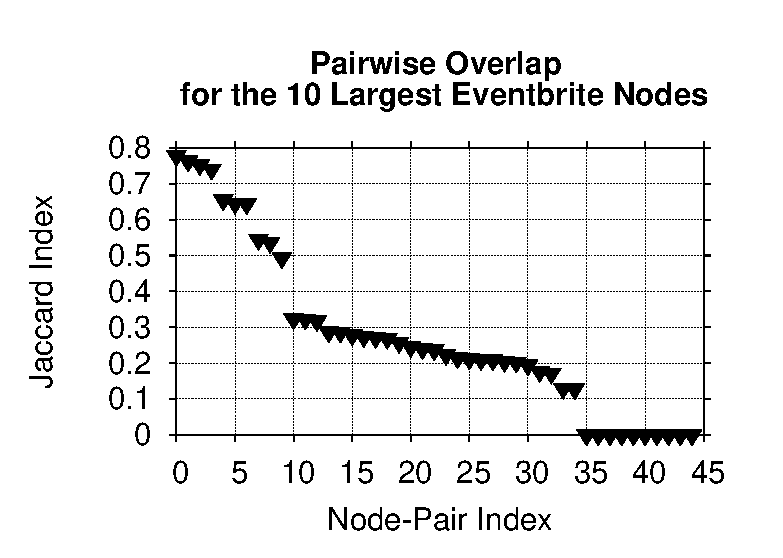
\includegraphics[clip,scale=0.5]{figs/overlaps.eps}
%	\vspace{-10pt}
%	\caption{Pairwise overlaps for the 10 most populous nodes.}
%	\label{fig:eventbriteover}
%	\vspace{-10pt}
%	\end{center}
%\end{figure}
%\fi
%\subsection{Contributions}
%\label{sec:contributions}
%Motivated by the examples above, we study the problem of crowdsourced entity extraction in the presence of long tail data. To effectively extract entities from the long tail we focus on {\em structured domains}. More precisely, we focus on domains described by a collection of attributes, each following a known {\em hierarchical structure}, i.e., we assume that for each attribute the corresponding hierarchy is known. Such hierarchies are usually dictated by the design of applications. \iftr Moreover, as controlling the overall extraction cost in large-scale applications is crucial we focus on {\em budgeted crowd entity extraction}. \fi
%
%We propose a novel algorithmic framework that exploits the structure of the domain to maximize the number of extracted entities under given budget constraints by targeting tail entities. In particular, we view the problem of entity extraction as a {\em multi-round adaptive optimization problem}. At  each round we exploit the information on extracted entities obtained by previous queries to adaptively select the crowd query that will maximize the {\em cost-gain} trade-off at each round. The gain of a query is defined as the {\em number of new unique entities extracted}. 
%
%We consider {\em generalized queries} that ask workers to provide us with entities from a domain $D$ and can also include an {\em exclude list}. In general such queries are of the type ``Give me $k$ more entities with attributes $\bar{X}$ that belong in domain $D$ and are not in $\{A, B, ...\}$''. Extending techniques from the species estimation and building upon the multi-armed bandits literature, we introduce a new methodology for estimating the gain for such generalized queries and show how the hierarchical structure of the domain can be exploited to increase the number of extracted entities. Our main contributions are as follows:
%
%\squishlist
%\item We formalize the notion of an exclude list for crowdsourced entity extraction queries and show how previously proposed gain estimators can be extended to handle such queries.
%\item We develop a new technique to estimate the gain of generalized entity extraction queries under the presence of little information, i.e., only when a small portion of the underlying entity population has been observed. We empirically demonstrate its effectiveness when extracting entities from sparse domains.
%\item We introduce an adaptive optimization algorithm that takes as input the gain estimates for different types of queries and identifies querying policies that maximize the total number of retrieved entities under given budget constraints. 
%\item Finally, we show that our techniques can effectively solve the problem of budgeted crowd entity extraction for large data domains on both real-world and synthetic data.
%\squishend

